\chapter{Categorical Statements}
\label{ch:catstatements}
\markright{Chap. \ref{ch:catstatements}: Categorical Statements}

\newglossaryentry{quantified categorical statement}
{
  name=quantified categorical statement,
  description={A statement that makes a claim about a certain quantity of the members of a class or group.}
}

\newglossaryentry{quantifier}
{
  name=quantifier,
  description={The part of a categorical sentence that specifies a portion of a class.}
}

\newglossaryentry{subject class}
{
  name=subject class,
  description={The first class named in a quantified categorical statement.}
}

\newglossaryentry{predicate class}
{
  name=predicate class,
  description={The second class named in a quantified categorical statement.}
  }

\newglossaryentry{copula}
{
  name=copula,
  description={The form of the verb ``to be'' that links subject and predicate.}
}

\newglossaryentry{quantity}
{
name=quantity,
description={The portion of the subject class described by a categorical statement. Generally ``some'' or ``none.''}
}

\newglossaryentry{universal}
{
name=universal,
description={The quantity of a statement that uses the quantifier ``all.''}
}

\newglossaryentry{particular}
{
name=particular,
description={The quantity of a statement that uses the quantifier ``some.''}
}

\newglossaryentry{quality}
{
name=quality,
description={The status of a categorical statement as affirmative or negative.}
}

\newglossaryentry{negative}
{
name=negative,
description={The quality of a statement containing a ``not'' or ``no.''}
}

\newglossaryentry{affirmative}
{
name=affirmative,
description={The quality of a statement without a ``not'' or a ``no.''}
}

\newglossaryentry{statement mood}
{
name=statement mood,
description={The classification of a categorical statement based on its quantity and quality.}
}

\newglossaryentry{mood-A statement}
{
name=mood-A statement,
description={A quantified categorical statement of the form ``All $S$ are $P$.''}
}

\newglossaryentry{mood-E statement}
{
name=mood-E statement,
description={A quantified categorical statement of the form ``No $S$ are $P$.''}
}

\newglossaryentry{mood-I statement}
{
name=mood-I statement,
description={A quantified categorical statement of the form ``Some $S$ are $P$.''}
}

\newglossaryentry{mood-O statement}
{
name=mood-O statement,
description={A quantified categorical statement of the form ``Some $S$ are not $P$.''}
}

\newglossaryentry{distribution}
{
name=distribution,
description={A property of the terms of a categorical statement that is present when the statement makes a claim about the whole term.}
}

\newglossaryentry{Venn diagram}
{
name=Venn diagram,
description={A diagram that represents categorical statements using circles that stand for classes.}
}

\newglossaryentry{translation key}
{
name=translation key,
description={A list that assigns English phrases or sentences to variable names. Also called a ``symbolization key''  or simply a ``dictionary.''}
}

\newglossaryentry{logically structured English}
{
name=logically structured English,
description={English that has been regimented into a standard form to make its logical structure clear and to remove ambiguity. A stepping stone to full-fledged formal languages.}
}

\newglossaryentry{standard form for a categorical statement}
{
name=standard form for a categorical statement,
description={A categorical statement that has been put into logically structured English, with the following elements in the following order: (1) The quantifiers ``all,'' ``some,'' or ``no''; (2) the subject term; (3) the copula ``are'' or ``are not''; and (4) the predicate term.}
}

\newglossaryentry{truth value}
{
  name=truth value,
  description={The status of a statement with relationship to truth. For  this textbook, this means the status of a statement as true or false}
}

\newglossaryentry{conversion}
{
name=conversion,
description={The process of changing a sentence by reversing the subject and predicate.}
}

\newglossaryentry{complement}
{
name=complement,
description={The class of everything that is not in a given class.}
}

\newglossaryentry{obversion}
{
name=obversion,
description={The process of transforming a categorical statement by changing its quality and replacing the predicate with its complement.}
}

\newglossaryentry{contraposition}
{
name=contraposition,
description={The process of transforming a categorical statement by reversing subject and predicate and replacing them with their complements.}
}

\section{Quantified Categorical Statements}
\label{sec:qcatstatements}

Back in Chapter \ref{ch:what_is_logic}, we saw that a statement was a unit of language that could be true or false (a proposition is the ``content'' of a statement). In this chapter and the next we are going to look at a particular kind of statement, called a \emph{quantified categorical} statement, and begin to develop a formal theory of how to create arguments using these statements. This kind of logic is generally called ``categorical'' or ``Aristotelian'' logic, because it was originally invented by the great logician and philosopher Aristotle in the fourth century \textsc{bce}. This kind of logic was the preeminent logical formalism throughout Europe, Africa, and the Middle East for 20 centuries afterward, and was expanded in all kinds of fascinating ways by Muslim and Catholic scholars, some of which we will look at here.

Consider the following propositions:

\begin{enumerate}[label=(\alph*)]
    \item \label{itm:dogs} All dogs are mammals.
    \item \label{itm:physicists} Most physicists are smart.
    \item \label{itm:politicians} Few politicians are honest.
    \item \label{itm:no_dogs} No dogs are cats.
    \item \label{itm:americans} Some Americans are doctors.
    \item \label{itm:adults}Some adults are not logicians.
    \item \label{itm:canadians} Thirty percent of Canadians speak French.
    \item \label{itm:chair} One chair is missing.
\end{enumerate}



These are all examples of quantified categorical statements. A  \textsc{\gls{quantified categorical statement}} \label{def:quantified_categorical_statement} is a statement that makes a claim about a certain quantity of the members of a class or group. (Sometimes we will just call these ``categorical statements'') Statement \ref{itm:dogs}, for example, is about the class of dogs and the class of mammals. These statements make no mention of any particular members of the categories or classes or types they are about. The propositions are also \textit{quantified} in that they state \textit{how many} of the things in one class are also members of the other. For instance, statement \ref{itm:physicists} talks about \textit{most} physicists, while statement \ref{itm:politicians} talks about \textit{few} teachers.

Categorical statements can be broken down into four parts: the quantifier, the subject term, the predicate term, and the copula. The \textsc{\gls{quantifier}} \label{def:quantifier} is the part of a categorical sentence that specifies a portion of a class. It is the ``how many'' term. The quantifiers in the sentences above are all, most, few, no, some, thirty percent, and one. Notice that the ``no'' in sentence \ref{itm:no_dogs} counts as a quantifier, the same way zero counts as a number. The subject and predicate terms are the two classes the statement talks about. The \textsc{\gls{subject class}} \label{def:subject_class} is the first class mentioned in a quantified categorical statement, and the \textsc{\gls{predicate class}} \label{def:predicate_class} is the second. In sentence \ref{itm:americans}, for instance, the subject class is the class of Americans and the predicate class is the class of doctors.  The \textsc{\gls{copula}} \label{def:copula} is simply the form of the verb ``to be'' that links subject and predicate. Notice that the quantifier is always referring to the subject. The statement ``Thirty percent of Canadians speak French'' is saying something about a portion of Canadians, not about a portion of French speakers.

Sentence \ref{itm:canadians} is a little different than the others. In sentence \ref{itm:canadians} the subject is the class of Canadians and the predicate is the class of people who speak French. That's not quite the way it is written, however. There is no explicit copula, and instead of giving a noun phrase for the predicate term, like ``people who speak French,'' it has a verb phrase, ``speak French.'' If you are asked to identify the copula and predicate for a sentence like this, you should say that the copula is implicit and transform the verb phrase into a noun phrase. You would do something similar for sentence \ref{itm:chair}: the subject term is ``chair,'' and the predicate term is ``things that are missing.'' We will go into more detail about these issues in Section \ref{sec:transformation}.


\begin{figure}
\begin{tikzpicture}
    \node[ellipse,draw=black] (a) at (0,0) {Some};
    \node[ellipse,draw=black] (b) at (2.2,0) {Americans};
    \node[ellipse,draw=black] (c) at (4.2,0) {are};
    \node[ellipse,draw=black] (d) at (5.8,0) {doctors.};
    \node[] (e) at (-1,1) {quantifier};
    \node[] (f) at (1,-1) {subject};
    \node[] (g) at (3,1) {copula};
    \node[] (h) at (5,-1) {predicate};
    \draw[->] (e) edge (a);
    \draw[->] (f) edge (b);
    \draw[->] (g) edge (c);
    \draw[->] (h) edge (d);
\end{tikzpicture}
\caption{Parts of a quantified categorical statement.}
\label{fig:Partsofacategoricalstatement}
\end{figure}

In the previous chapter we noted that formal logic achieves content neutrality by replacing some or all of the ordinary words in a statement with symbols. For categorical logic, we are only going to be making one such substitution. Sometimes we will replace the classes referred to in a quantified categorical statement with capital letters that act as variables. Typically we will use the letter $S$ when referring to the class in the subject term and $P$ when referring to the predicate term, although sometimes more letters will be needed. Thus the sentence ``Some Americans are doctors,'' above, will sometimes become ``Some $S$ are $P$.'' The sentence ``No dogs are cats'' will sometimes become``No $S$ is $P$.''

\section{Quantity, Quality, Distribution, and Venn Diagrams}\label{sec:QQDVD}

Ordinary English contains all kinds of quantifiers, including the counting numbers themselves. In this chapter and the next, however, we are only going to deal with the quantifiers: ``all,'' ``no,'' and ``some.'' We are restricting ourselves to the quantifiers ``all'' and ``some'' because they are the ones that can easily be combined to create valid arguments using the system of logic that was invented by Aristotle. We will deal with other quantifiers in Chapter \ref{ch:inductivelogic}, on induction. There we will talk about much more specific quantified statements, like ``Thirty percent of Canadians speak French,'' and do a little bit of work with modern statistical methods.

The quantifier used in a statement is said to give the \textsc{\gls{quantity}} \label{def:Quantity} of the statement. Statements with the quantifier ``All'' are said to be ``\textsc{\gls{universal}}'' and those with the quantifier ``some'' are said to be ``\textsc{\gls{particular}}.''

Here ``some'' will just mean ``at least one.'' So, ``some people in the room are standing'' will be true even if there is only one person standing. Also, because ``some'' means ``at least one,'' it is consistent with the corresponding ``all'' statement. If I say ``some people in the room are standing'' it might actually be that \emph{all} people in the room are standing, because if all people are standing, then at least one person is standing. This can sound a little weird, because in ordinary circumstances, you wouldn't bother to point out that something applies to some members of a class when, in fact, it applies to all of them. It sounds odd to say ``\emph{some} dogs are mammals,'' when in fact they \emph{all} are. Nevertheless, when ``some'' means ``at least one'' it is perfectly true that some dogs are mammals.


In addition to talking about the quantity of statements, we will talk about their \textsc{\gls{quality}}. \label{def:quality} The quality of a statement refers to whether the statement is negated. Statements that include the words ``no'' or ``not'' are \textsc{\gls{negative}}, and other statements are \textsc{\gls{affirmative}}. Combining quantity and quality gives us four basic types of quantified categorical statements, which we call the \textsc{\glspl{statement mood}} or just ``moods.'' The four moods are labeled with the letters A, E, I, and O. Statements that are universal and affirmative are \textsc{\glspl{mood-A statement}}. Statements that are universal and negative are \textsc{\glspl{mood-E statement}}. Particular and affirmative statements are \textsc{\glspl{mood-I statement}}, and particular and negative statements are \textsc{\glspl{mood-O statement}}. (See Table \ref{tab:moods}.)


Aristotle didn't actually use those letters to name the kinds of categorical propositions. His later followers writing in Latin came up with the idea. They remembered the labels because the ``A'' and the ``I'' were in the Latin word ``\textbf{a}ff\textbf{i}rmo,'' (``I affirm'') and the ``E'' and the ``O'' were in the Latin word ``n\textbf{e}g\textbf{o}'' (``I deny'').

\begin{table}[t]
\begin{tabu}{p{.1\linewidth}p{.3\linewidth}p{.3\linewidth}}
  \underline{Mood}& \underline{Form} & \underline{Example} \\
A & All $S$ are $P$.      & All dogs are mammals. \\
E & No $S$ are $P$.       & No dogs are reptiles. \\
I & Some $S$ are $P$.     & Some birds can fly. \\
O & Some $S$ are not $P$. & Some birds cannot fly.\\
\end{tabu}
\caption{The four moods of categorical statements}
\label{tab:moods}
\end{table}



The \textsc{\gls{distribution}} of a categorical statement refers to how the statement describes its subject and predicate class. A term in a sentence is said to be distributed \label{def:Distribution} if a claim is being made about the whole class. In the sentence ``All dogs are mammals,'' the subject class, dogs, is distributed, because the quantifier ``All'' refers to the subject. The sentence is asserting that every dog out there is a mammal. On the other hand, the predicate class, mammals, is not distributed, because the sentence isn't making a claim about all the mammals. We can infer that at least some of them are dogs, but we can't infer that all of them are dogs. So in mood-A statements, only the subject is distributed.

On the other hand, in an $I$ sentence like ``Some birds can fly'' the subject is not distributed. The quantifier ``some'' refers to the subject, and indicates that we are not saying something about all of that subject. We also aren't saying anything about all flying things, either. So in mood-I statements, neither subject nor predicate is distributed.

Even though the quantifier always refers to the subject, the predicate class can be distributed as well. This happens when the statement is negative. The sentence ``No dogs are reptiles'' is making a claim about all dogs: they are all not reptiles. It is also making a claim about all reptiles: they are all not dogs. So mood-E statements distribute both subject and predicate. Finally, negative particular statements (mood-O) have only the predicate class distributed. The statement ``some birds cannot fly'' does not say anything about all birds. It does, however say something about all flying things: the class of all flying things excludes some birds.

The quantity, quality, and distribution of the four forms of a categorical statement are given in Table \ref{tab:quantity}. The general rule to remember here is that universal statements distribute the subject, and negative statements distribute the predicate.


\begin{table*}
\begin{tabu} to \textwidth {X[0.6] X[1.4] X[1] X[1.2] X[2.4] }
 \textbf{Mood} & \textbf{Form} &  \textbf{Quantity} & \textbf{Quality} & \textbf{Terms Distributed} \\
A & All $S$ are $P$      & Universal  & Affirmative & S\\
E & No $S$ are $P$       & Universal  & Negative    & S and P\\
I & Some $S$ are $P$     & Particular & Affirmative & None\\
O & Some $S$ are not $P$ & Particular & Negative    & P \\
\end{tabu}
\caption{Quantity, quality, and distribution.}
\label{tab:quantity}
\end{table*}

In 1880, the English logician John Venn published two essays on the use of diagrams with circles to represent categorical propositions.\footnote{See \parencite{Venn1880a}, \parencite{Venn1880b}} Venn noted that the best use of such diagrams so far had come from the brilliant Swiss mathematician Leonhard Euler, but they still had many problems, which Venn felt could be solved by bringing in some ideas about logic from his fellow English logician George Boole. Although Venn only claimed to be building on the long logical tradition he traced, since his time these kinds of circle diagrams have been known as \textsc{\glspl{Venn diagram}}.

\begin{figure}
\begin{center}
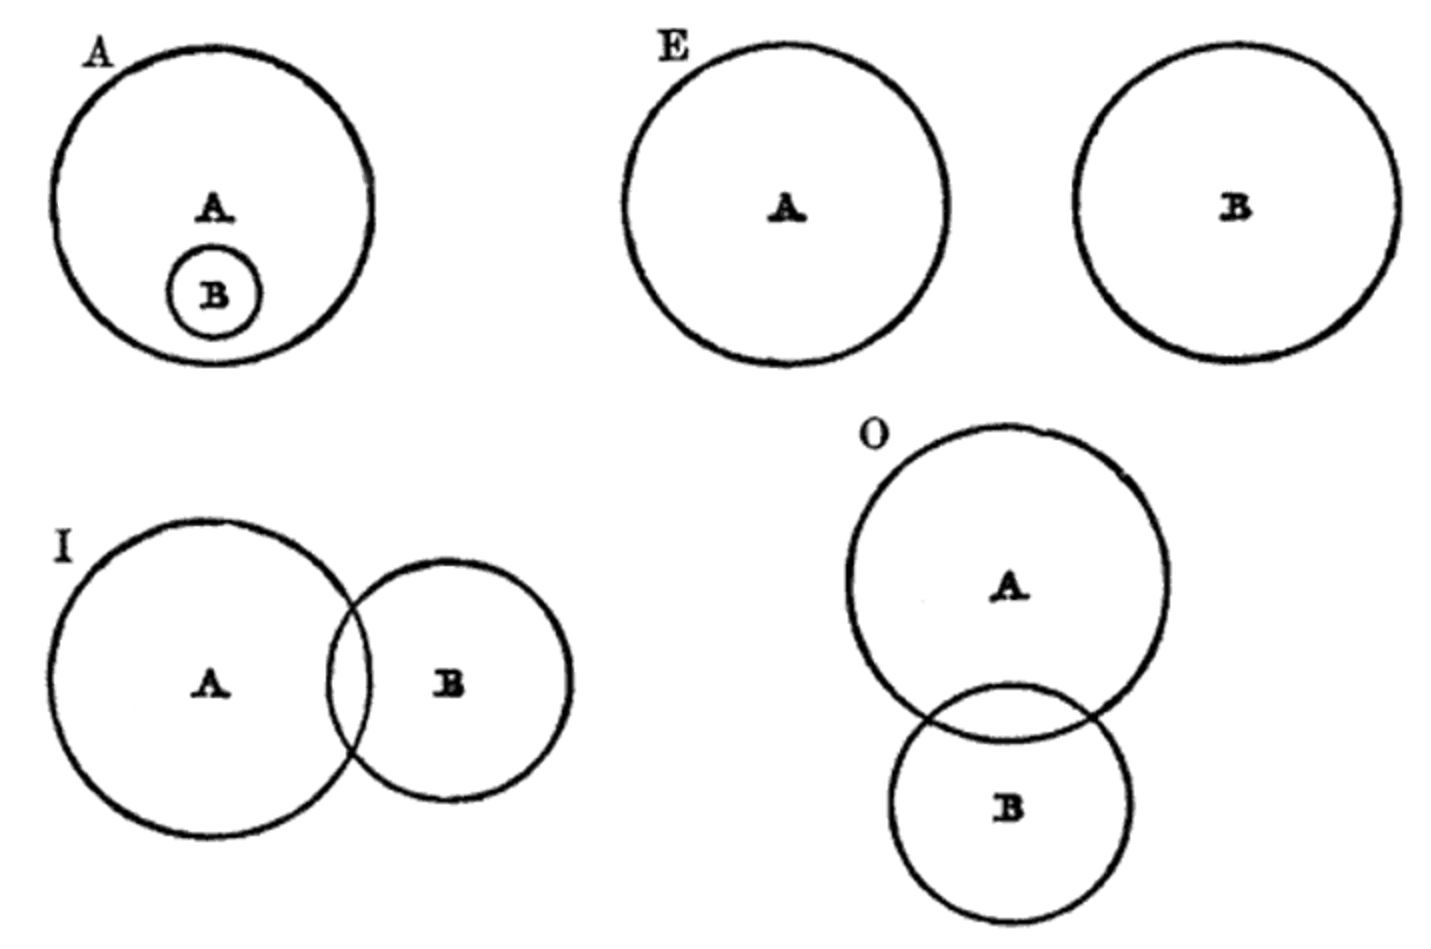
\includegraphics[width=0.8\textwidth]{euler_diagrams}
\end{center}
\caption{Euler diagrams from Scottish philosopher William Hamilton's \textit{Lectures on Logic}.}
\label{fig:euler_circles}
\end{figure}

In this section we are going to learn to use Venn diagrams to represent our four basic types of categorical statement. Later in this chapter, we will find them useful in evaluating arguments.

Let us start with a statement in mood A: ``All $S$ are $P$.'' We are going to use one circle to represent $S$ and another to represent $P$. There are a couple of different ways we could draw the circles if we wanted to represent ``All $S$ are $P$.'' One option would be to draw the circle for $S$ entirely inside the circle for $P$, as in the Euler diagram in the top-left of figure~\ref{fig:euler_circles}.

\begin{figure}[!ht]
\begin{center}
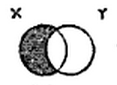
\includegraphics[width=0.6\textwidth]{OriginalVenn}
\end{center}
\caption{Venn's original diagram for an mood-A statement from \parencite{Venn1880a}. Screencap from Google Books by J. Robert Loftis.}
\end{figure}


It is clear from the top left Euler diagram in figure~\ref{fig:euler_circles} that all $B$ are in fact $A$. And outside of college logic classes, you may have seen people use a diagram like this to represent a situation where one group is a subclass of another. You may have even seen people call concentric circles like this a Venn diagram. But Venn did not think we should put one circle entirely inside the other if we just want to represent ``All $S$ is $P$.'' Technically speaking figure \ref{fig:euler_circles} shows Euler circles, not Venn diagrams.

Venn pointed out that the circles in the top left of figure \ref{fig:euler_circles} don't just say that ``All $B$ are $A$.'' They also say that ``All $A$ are $B$'' is false. But we don't necessarily know that if we have only asserted ``All $B$ are $A$.'' The statement ``All $B$ are $A$'' leaves it open whether the $B$ circle should be smaller than or the same size as the $A$ circle.

Venn suggested that to represent just the content of a single proposition, we should always begin by drawing partially overlapping circles. This means that we always have spaces available to represent the four possible ways the terms can combine. Thus, for a single sentence we should always draw the diagram as in figure~\ref{fig:basicvenn}.

\begin{marginfigure}
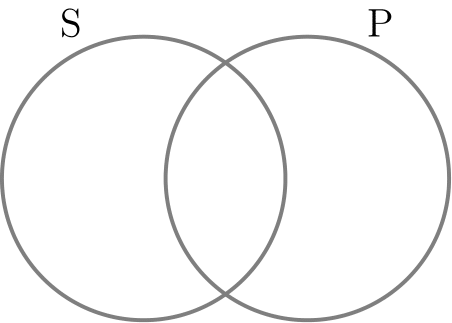
\includegraphics{2venn1}
\caption{A basic Venn diagram.}
\label{fig:basicvenn}
\end{marginfigure}

To return to our initial question, suppose we want to represent the sentence ``All $S$ is $P$.'' using Venn diagrams. To do so we will shade the region of $S$ that does not overlap with $P$. This tells us that the left-hand side of S is empty and so everything that has property $S$ must also have property $P$. (See figure~\ref{fig:mooda}.)

\begin{marginfigure}
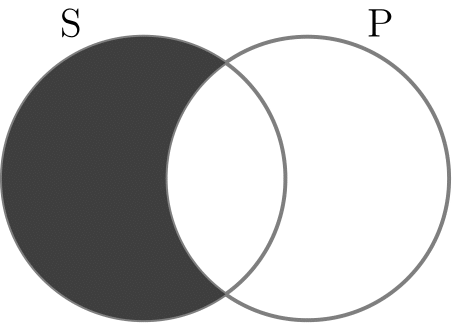
\includegraphics{2venn2}
\caption{A Venn diagram for a mood-A sentence.}
\label{fig:mooda}
\end{marginfigure}

If we want to say that something does exist in a region, we put an ``x'' in it. The diagram for ``Some $S$ are $P$'' is in figure~\ref{fig:moodi}.

\begin{marginfigure}
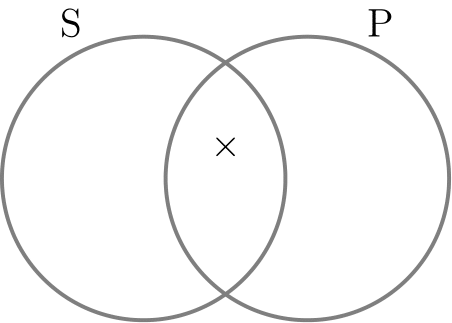
\includegraphics{2venn5}
\caption{A Venn diagram for a mood-I sentence.}
\label{fig:moodi}
\end{marginfigure}


If a region of a Venn diagram is blank, if it is neither shaded nor has an x in it, it could go either way. Maybe such things exist, maybe they do not.

The Venn diagrams for all four basic forms of categorical statements are in figure \ref{fourvenns}. Notice that when we draw diagrams for the two universal forms, A and E, we do not draw any x's. For these forms we are only ruling out possibilities, not asserting that things actually exist. This is part of what Venn learned from Boole, and we will see its importance in chapter \ref{ch:existentialimport}.

\begin{figure}[!ht]
\begin{minipage}[t]{0.4\textwidth}\centering
    \textbf{``All S is P.''}
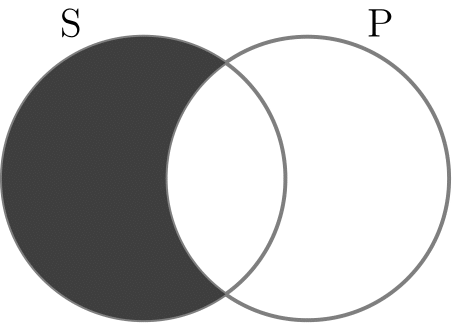
\includegraphics{2venn2}
\end{minipage}\hspace{1cm}
\begin{minipage}[t]{0.4\textwidth}\centering
    \textbf{``No S is P.''}
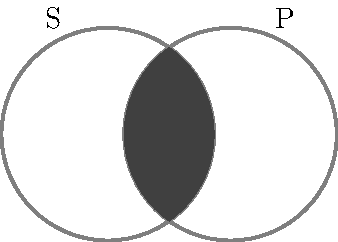
\includegraphics{2venn4}
\end{minipage}

\vspace{1cm}

\begin{minipage}[t]{0.4\textwidth}\centering
    \textbf{``Some S is P.''}
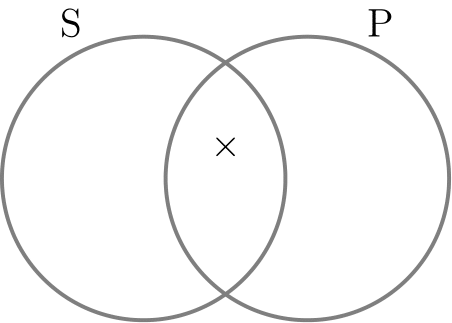
\includegraphics{2venn5}
\end{minipage}\hspace{1cm}
\begin{minipage}[t]{0.4\textwidth}\centering
    \textbf{``Some S is not P.''}
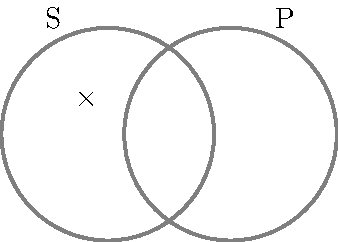
\includegraphics{2venn6}
\end{minipage}

\vspace{1cm}

\caption{Venn diagrams for all four categorical moods.}
\label{fig:fourvenns}
\end{figure}


Finally, notice that so far, we have only been talking about categorical statements involving the variables $S$ and $P$. Sometimes, though, we will want to represent statements in regular English. To do this, we will include a key saying what the variables $S$ and $P$ represent in this case. We will call a list that assigns English phrases or sentences to variable names a \textsc{\gls{translation key}}.\label{def:translation_key} These are sometimes also called ``symbolization keys'' or simply just ``dictionaries.'' As our logical systems get more complicated, the symbolization keys will get more complicated. For now, though, they just consist of a note saying what the $S$ and $P$ stand for. For instance, this is the diagram for ``No dogs are reptiles.''


\section{Transforming English into Logically Structured English} \label{sec:transformation}

Because the four basic forms are stated using variables, they have a great deal of generality. We can expand on that generality by showing how many different kinds of English sentences can be represented as sentences in our four basic forms. We already touched on this a little in section \ref{sec:qcatstatements}, when we look at sentences like ``Thirty percent of Canadians speak French.'' There we saw that the predicate was not explicitly a class. We needed to change ``speak French'' to ``people who speak French.'' In this section, we are going to expand on that to show how ordinary English sentences can be transformed into something we will call ``logically structured English.'' \textsc{\gls{logically structured English}} \label{def:LSE} is English that has been put into a standardized form that allows us to see its logical structure more clearly and removes ambiguity.  Doing this is a step towards the creation of formal languages, which we will start doing in Chapter \ref{ch:SL}.

Transforming English sentences into logically structured English is fundamentally a matter of understanding the meaning of the English sentence and then finding the logically structured English statements with the same or similar meaning. Sometimes this will require judgment calls. English, like any natural  language, is fraught with ambiguity. One of our goals with logically structured English is to reduce the amount of ambiguity. Clarifying ambiguous sentences will always require making judgments that can be questioned. Things will only get harder when we start using full blown formal languages in Chapter \ref{chap:SL}, which are supposed to be completely free of ambiguity.

To transform a quantified categorical statement into logically structured English, we have to put all of its elements in a fixed order and be sure they are all of the right type. All statements must begin with the quantifies ``All'' or ``Some'' or the negated quantifier ``No.'' Next comes the subject term, which must be a plural noun, a noun phrase, or a variable that stands for any plural noun or noun phrase. Then comes the copula ``are'' or the negated copula ``are not.'' Last is the predicate term, which must also be a plural noun or noun phrase. We also specify that you can only say ``are not'' with the quantifier ``some,'' that way the universal negative statement is always phrased ``No $S$ are $P$,'' not ``All S are not $P$.'' Taken together, these criteria define the \textsc{\gls{standard form for a categorical statement}} in logically structured English. \label{def:standard_form_cat_statement}

The subsections below identify different kinds of changes you might need to make to put a statement into logically structured English. Sometimes translating a sentence will require using multiple changes.

\subsection{Change the Predicate into a Noun Phrase}
\label{subsec:predicate_noun_phrase}
In section \ref{sec:qcatstatements} we saw that ``Some Canadians speak French'' has a verb phrase ``speaks French'' instead of a copula and a plural noun phrase. To transform these sentences into logically structured English, you need to add the copula and turn all the terms into plural nouns or plural noun phrases. Adding a plural noun phrase means you have to come up with some category, like ``people'' or ``animals.'' When in doubt, you can always use the most general category, ``things.'' Below are some examples

\begin{table}
\begin{longtabu}{p{.5\linewidth}p{.5\linewidth}}
\underline{English} &
\underline{Logically Structured English} \\
\endhead
No cats bark. &
No cats are animals that bark.  \\

All birds can fly. &
All birds are animals that can fly.  \\

Some thoughts should be left unsaid. &
Some thoughts are things that should be left unsaid.
\end{longtabu}
\end{table}

\noindent Sometimes English sentences will have a copula and an adjective or adjective phrase as the predicate. These need to be changed to noun phrases, just as the verb phrases did.

\begin{table}
\begin{longtabu}{p{.5\linewidth}p{.5\linewidth}}
\underline{English} &
\underline{Logically Structured English}  \\
\endhead
Some roses are red. &
Some roses are red flowers. \\

Football players are strong. &
All football players are strong persons. \\

Some words are hurtful. &
Some words are hurtful things.
\end{longtabu}
\end{table}

\noindent Again, you will have to come up with a category for the predicate, and when it doubt, you can just use ``things.''

\subsection{Standardize the Quantifier}
\label{subsec:standardize_quantifier}

English has a wide variety of ways to express quantity. We need to reduce all of these to either ``all'' or ``some,'' plus negations.  Here are some examples:

\begin{fullwidth}
\begin{longtabu}{p{.5\linewidth}p{.5\linewidth}}
\underline{English} &
\underline{Logically Structured English} \\
\endhead

Most people with a PhD in psychology are female. &
Some people with a PhD in psychology are female. \\

Among the things that Sylvia inherited was a large mirror &
Some things that Sylvia inherited were large mirrors\\

There are Americans that are doctors. &
Some Americans are doctors. \\

At least a few Americans are doctors.&
Some Americans are doctors. \\

A man is walking down the street. &
Some men are things that are walking down the street.\\


Every day is a blessing. &
All days are blessings. \\

Whatever is a dog is not a cat. &
No dogs are cats. \\

Not a single dog is a cat. &
No dogs are cats. \\

Take nothing for granted &
No things are things that should be taken for granted \\

Something is rotten in Denmark &
Some things are things that are rotten in Denmark\\

Everything is coming up roses &
All things are things that are coming up roses\\


``What does not destroy me, makes me stronger.'' --Friedrich Nietzsche &
All things that do not destroy me are things that make me stronger. \\


\end{longtabu}
\end{fullwidth}

Notice in the last case we are losing quite a bit of information when we transform the sentence into logically structured English. ``Most'' means more that fifty percent, while ``some'' could be any percentage less than a hundred. This is simply a price we have to pay in creating a standard logical form. As we will see when we move to constructing artificial languages in Chapter \ref{chap:SL}, no logical language has the expressive richness of a natural language.

Sometimes universal statements in English don't have an explicit quantifier. Instead they use a plural noun or indefinite article to express generality.

\begin{table}
\begin{longtabu}{p{.5\linewidth}p{.5\linewidth}}
\underline{English} &
\underline{Logically Structured English} \\
\endhead
Boots are footwear. & All boots are footwear.\\
Giraffes are tall. & All giraffes are tall things.\\
A dog is not a cat. & No dogs are cats.\\

A lion is a fierce creature. &
All lions are fierce creatures.\\

\end{longtabu}
\end{table}

\noindent Notice that in the second sentence we had to make two changes, adding both the words ``All'' and ``things.''

In the last two sentences, the indefinite article ``a'' is being used to create a kind of generic sentence. Not all sentences using the indefinite article work this way. The list before this one included the example ``A man is walking down the street.'' This sentence is not talking about all men generically. It is talking about a specific man whose identity is unknown. Here the indefinite article is being used like a nonstandard version of the quantifier ``some,'' which is why it appeared in the earlier list. You will have to use your good judgment and understanding of context to know when the indefinite article is being used like the word ``all'' and when it is being used like the word ``some.''

You may be someone who interprets these indefinite sentences slightly differently. Sometimes, English speakers say things like, ``Dogs bark.'' to mean something like, ``\emph{Most} dogs are things that bark.'' or ``Typically, dogs are things that bark.'' Indefinite articles and generic sentences like this are quintessentially \emph{vague} sentences. Because we do not have a way to formalize the quantifier `most' we are going to translate generics as expressing a universal quantity. So, ``Dogs bark.'' will become ``All dogs are things that bark.'' More advanced categorical logics that have an infinite number of quantifiers attempt to translate the detail of these generics more precisely, but we won't worry about that for now.

English also uses specialized adverbial phrases as quantifiers for people, places and times. If we want to talk about all people, we use a specialized quantifier like ``everyone,'' ``someone'' or ``no one.'' We use ``everywhere,'' ``somewhere,'' and ``nowhere'' for places, and ``always,'' ``sometimes,'' and ``never'' for times.  All of these need to be transformed into using the simple quantifiers ``all'' or ``some,'' plus negations.

\begin{fullwidth}
\tabulinesep=1.25ex
\begin{longtabu}{p{.5\linewidth}p{.5\linewidth}}
\underline{English} &
\underline{Logically Structured English} \\
\endhead
Someone in America is a doctor. &
Some Americans are doctors. \\

Not everyone who is an adult is a logician. &
Some adults are not logicians. \\

``Whenever you need me, I'll be there.'' -- Michael Jackson &
All times that you need me are times that I will be there. \\

``We are never, ever, ever getting back together.'' -- Taylor Swift &
No times are times when we will get back together.\\

``Whoever fights with monsters should be careful lest he thereby become a monster.'' --Friedrich Nietzsche &
All persons who fight with monsters are persons who should be careful lest they become a monster.\\

\end{longtabu}
\end{fullwidth}

\subsection{Standardize Alternative Universal Forms}
\label{subsec:alternative_universals}

Many constructions in English can be represented as universal statements in Logically Structured English, either affirmative (A) or negative (E)

For instance, it turns out that statements about individual people or specific objects can be represented by A or E statements. This is not something Aristotle originally noticed. For him a statement like ``Socrates is mortal,'' for Aristotle, were neither universal nor particular. They were a third class he called ``singular.'' The power of categorical logic was expanded considerably when it was realized singular statements can converted into universal statements. The trick is to add a phrase like ``All things identical to\ldots'' to our singular sentence. Essentially we are adding a universal quantifier that only picks out one specific object.

\begin{table*}[!ht]
\begin{longtabu}{p{.5\linewidth}p{.5\linewidth}}
\underline{English} & \underline{Logically Structured English} \\
\endhead
Socrates is mortal. & All persons identical with Socrates are mortal. \\
The Empire State Building is tall. & All things identical to The Empire State Building are tall things. \\
Ludwig was not happy. & No people identical with Ludwig are happy people. \\

\end{longtabu}
\end{table*}


%
%\subsection{``It Is False That''}
%
%In English, we can say ``It is false that \ldots'' or ``It is not the case that \ldots'' to indicate that a statement is false. A lawyer, for instance, might say ``It is not the case that you signed the consent form before the doctor did the procedure.'' In logically structured English, we can make these simpler by converting the negated proposition to its contradictory. A negated A statement will become an O statement, and vice versa. Likewise a negating E statement will become and I statement, and vice versa. See the examples below. This time we have marked their form A, E, I or O, with a ``not-'' for the cases where they are negated.
%
%\begin{tabu}{p{.5\linewidth}p{.5\linewidth}}
%\underline{English} &
%\underline{Logically Structured English} \\
%
%\textbf{not-A}: It is not the case that all dogs are pets &
%\textbf{O}: Some dogs are not pets.\\
%
%\textbf{not-I}: It is not the case that some dogs are reptiles &
%\textbf{E}: No dogs are reptiles\\
%
%\textbf{not-E}: It is not the case that no dogs are pets &
%\textbf{I}: Some dogs are pets \\
%
%\textbf{not-O}: It is not the case that some dogs are not mammals &
%\textbf{A}: All dogs are mammals.
%\end{tabu}

Another kind of statement that can be transformed into a universal statement is a conditional. A conditional is a statement of the form ``If \ldots then \ldots.'' They will become a big focus of our attention starting in Chapter \ref{chap:SL} when we begin introducing modern formal languages. They are not given special treatment in the Aristotelian tradition, however. Instead, where we can, we just treat them as categorical generalizations:

\begin{table*}
\begin{longtabu}{p{.5\linewidth}p{.5\linewidth}}
\underline{English} & \underline{Logically Structured English} \\
\endhead
If something is a cat, then it is a felines. & All cats are feline.\\
If something is a dog, then it's not a cat. & No dogs are cats. \\
\end{longtabu}
\end{table*}

The word ``only'' is used in a couple of different constructions in English that can be represented as universal statements. The first kind are called ``exclusive propositions.'' These are statements that say the subject excludes everything except what is in the predicate. For instance the sentence ``Only people over 21 may drink'' says that the class of people who may drink excludes everyone except those who are over 21. In English exclusive propositions are created using the words ``only,'' ``none but,'' or ``none except.'' These statements become A statements when translated into logically structured English. So ``Only people over 21 may drink'' becomes ``If you may drink, you  are over 21.'' It is important to see that in each case these words are used to introduce the predicate, not the subject. In the sentence ``Only people over 21 may drink,'' the term ``people over 21'' is actually the  predicate, and ``people who may drink'' is the subject.

\begin{table*}
\begin{longtabu}{p{.5\linewidth}p{.5\linewidth}}
\underline{English} & \underline{Logically Structured English} \\
\endhead
Only people over 21 may drink. & All people who drink are over 21.\\
No one, except those with a ticket, may enter the theater. & All people who enter the theater have a ticket. \\
None but the strong survive. & All people who survive are strong people. \\
\end{longtabu}
\end{table*}

Sentences with ``The only'' are a little different than sentences regular exclusive propositions, which just have ``only'' in them. The sentence ``Humans are the only animals that talk on cell phones'' should be translated as ``All animals who talk on cell phones are humans.'' In this sentence, ``the only'' introduces the subject, rather than the predicate. The statement still asserts that the subject excludes everything except what is in the predicate, and we still represent them using mood A statements.

\begin{table*}
\begin{longtabu}{p{.5\linewidth}p{.5\linewidth}}
\underline{English} & \underline{Logically Structured English} \\
\endhead
Humans are the only animals who talk on cell phones. & All animals who talk on cell phones are human.\\
Shrews are the only venomous mammal in North America. & All venomous mammals in North America are shrews.\\
\end{longtabu}
\end{table*}

Transforming sentences into \gls{logically structured English} requires judgment and attention to the nuances of meaning in English. You must be able to recognize which of the transformations describe above needs to be applied and apply it correctly. One frequent mistake by people starting out is to overgeneralize. We saw at the start of the subsection on alternative universal forms that singular propositions can be turned into universal propositions by adding the phrase ``Things identical to \ldots'' Once you get in the habit of doing this, it becomes tempting to add the phrase ``things identical to \ldots'' to everything, even when it isn't necessary or doesn't make sense. The sentence ``Fido is a dog'' should become ``all things identical to Fido are dogs'' in logically structured English, because ``Fido'' is a singular term referring to an individual dog. But with the sentence ``dogs are mammals,'' you do not need to add the phrase ``All things identical to\ldots'', because ``dogs'' is already a collective noun, not an individual.

The same is true for the phrases we use to transform adjective and verb phrases into noun phrases. The sentence ``No cats bark'' has to be changed, because ``bark'' is a verb, so it becomes ``No cats are animals that bark'' in Logically Structured English. But the sentence ``No cats are reptiles'' already has a noun, ``reptiles,'' for a predicate, so you do not need to transform it into ``No cats are animals that are reptiles.'' The key is not only knowing when to use the transformations we describe, but knowing when not to use them.



\section*{Key Terms}
\begin{multicols}{2}
\begin{sortedlist}
\sortitem{Quantified categorical statement}{}
\sortitem{Quantifier}{}
\sortitem{Subject class}{}
\sortitem{Predicate class}{}
\sortitem{Copula}{}
\sortitem{Truth value}{}
\sortitem{Mood-A statement}{}
\sortitem{Mood-E statement}{}
\sortitem{Mood-I statement}{}
\sortitem{Mood-O statement}{}
\sortitem{Quantity}{}
\sortitem{Quality}{}
\sortitem{Logically structured English}{}
\sortitem{Distribution}{}
\sortitem{Complement}{}
\sortitem{Converse}{}
\sortitem{Obverse}{}
\sortitem{Contraposition}{}
\sortitem{Contradictories}{}
\sortitem{Contraries}{}
\sortitem{Square of opposition}{}
\sortitem{Subcontraries}{}
\sortitem{Subalternation}{}
\sortitem{Existential import}{}
\sortitem{Vacuous truth}{}
\sortitem{Venn diagram}{}
\sortitem{Standard form categorical statement}{}
\sortitem{Universal}{}
\sortitem{Particular}{}
\sortitem{Affirmative}{}
\sortitem{Negative}{}
\sortitem{Translation key}{}
\end{sortedlist}
\end{multicols}
